\newcommand{\Versione}{1.0}%Versione Finale
\newcommand{\Data}{2013-01-21}%Data di creazione
%\newcommand{\TipoDocumento}{Relazione finale sullo stage}

\documentclass[a4paper]{article}
\usepackage[utf8x]{inputenc}
\usepackage[italian]{babel}
\usepackage{fancyhdr}
%%pacchetto per il float delle immagini
\usepackage{float}
\usepackage{sidecap,caption}
\usepackage{eurofont}
\usepackage{lastpage}
\usepackage{graphicx}
%\usepackage{fullpage}
\usepackage{setspace}
\usepackage{textcomp}
\usepackage{booktabs}
\usepackage{color}
\usepackage{lscape}
\usepackage{hyperref}
\hypersetup{colorlinks=true, linkcolor=blue, anchorcolor=red, urlcolor=blue}
\usepackage{longtable}
\usepackage{tabularx}
\usepackage{abstract}
\usepackage{appendix}
\usepackage{multicol}
\usepackage{bmpsize}
%%%%%%%%%%%%%%%needed for glossario%%%%%%%%%
%\usepackage{guit}

%\usepackage[acronym]{glossaries}
%\newglossaryentry{parola}{name=parola,description={Si spiega da sé}}
%\newacronym{guit}{\GuIT{}}{Gruppo Utilizzatori Italiani di \TeX{}}
%\addto\captionsitalian{\renewcommand{\glossaryname}{Glossario}}
%\makeglossaries
%%%%%%%%%%%%%%%%%%%%%%%%%fine need glossario
%%%%%%%%%%%glossario prova 2
\usepackage{glossaries}
\addto\captionsitalian{\renewcommand{\glossaryname}{Glossario}}
\newglossaryentry{prova}{name=prova, description={parole a caso}}
\newglossaryentry{dematerializzazione} {name=dematerializzazione, description={processo che ha come obiettivo ultimo la creazione di un flusso di documenti digitali aventi pieno valore giuridico, che vada prima ad affiancare e poi, sul lungo periodo, a sostituire la normale documentazione cartacea presente negli archivi di qualunque attività pubblica o privata.}}
\makeglossaries
%%%%%%%%%%%%%% fine glossario prova 2
\usepackage[all]{hypcap}
\oddsidemargin=.15in
\evensidemargin=.15in
\textwidth=6in
%\topmargin=-.5in
\parindent=0in
%\headheight=1in
\pagestyle{fancy}
\lhead{
\bfseries {\Large \TipoDocumento}\\
\bfseries Versione: \Versione\\
}
\chead{}
\lhead{
%\includegraphics[scale=0.455]{../Logo&Header/SEVENTECH2.png}
}
%\lfoot{\bfseries \TipoDocumento{} v\Versione}
\cfoot{}
\rfoot{\thepage\ of \mypageref{LastPage}}
\newcommand*{\mypageref}[1]{
\hypersetup{linkcolor=black}\pageref{#1}\hypersetup{linkcolor=black}}
%\userpackage{lipsum}
\renewcommand{\footrulewidth}{0.4pt}
%\newcommand{\numref}[1]{\textsl{\nameref{#1} (\ref{#1})}}
%\newcommand{\NomeGruppo}{SevenTech}
%\newcommand{\Progetto}{''3DMob: Grafica 3D su device mobili''}
%\newcommand{\Prop}{Mentis s.r.l.}
%\newcommand{\Glossario}{Al fine di evitare incomprensioni dovute a possibili ambiguità del linguaggio, dei termini e acronimi utilizzati nei documenti, viene allegato il glossario contenuto nel file \emph{Glossario\_{}vX.Y.pdf}.
%Saranno in esso definiti e descritti tutti i termini marcati da una \underline{sottolineatura} nella documentazione fornita.}

%\newcommand{\Prodotto}{

%Il prodotto denominato 3DMob ha lo scopo di fornire un \underline{applicativo} in grado di interpretare \underline{oggetti 3D} a partire dai \underline{formati} \underline{3DS} o \underline{OBJ} e relativo file \underline{MTL}, permettendo all'\underline{utente} di applicare modifiche alla \underline{scena 3D} e di visualizzarne l'anteprima. Il prodotto dovrà successivamente consentire l'\underline{esportazione} del modello 3D nel \underline{formato} \underline{JSON} o \underline{XML}, in modo tale che sia immediatamente compatibile con le \underline{librerie} grafiche \underline{\underline{OpenGL} ES} 2.0, utilizzate nei \underline{device mobili}.
%  Tale formato dovrà essere conforme ai limiti impliciti delle \underline{librerie} grafiche \underline{OpenGL ES} 2.0, in modo che i file esportati possano essere immediatamente utilizzabili nei \underline{device mobili} che supportano tali librerie.

%}
\begin{document}
%\thispagestyle{empty}
%\begin{center}%\centerline{
%\includegraphics[scale=1.05]{../Logo&Header/logo_principale.png}}
%{\href{mailto:grupposwe2013@gmail.com}{\color[rgb]{0.39,0.37,0.38}grupposwe2013@gmail.com}}\\ [3pc]
%{\Huge {3DMob: Grafica 3D su device mobili}}\\[.5pc]
%\underline{\hspace{6in}}\\[3pc]
%{\Huge {\TipoDocumento}}\\[1pc]
%{\emph{Versione \Versione}}\\
%\end{center}
%\vspace{.3in}
\begin{titlepage}
 
\begin{center}
 
% Upper part of the page

\includegraphics[scale=.5]{logoBlack.png}
 
\textsc{\LARGE Università degli Studi di Padova}\\[1.5cm]
 
\textsc{\Large Dipartimento di Matematica\\[0.2cm] Corso di Laurea in Informatica}\\[0.8cm]
  
% Title
\\[0.8cm]{\Huge \doublespacing \bfseries \begin{spacing}{1}{Classificazione firme statiche utilizzando i Hidden~Markov~Models}\end{spacing}}
\\[2cm]

% Author and supervisor
\begin{minipage}{0.4\textwidth}
\begin{flushleft} \large
\emph{Relatore:} \\
Ch.mo Prof. Tullio \textsc{Vardanega}
\end{flushleft}
\end{minipage}
\begin{minipage}{0.4\textwidth}
\begin{flushright} \large
\emph{Laureando:}\\
Alexandru \textsc{Prigoreanu 1004887}
\end{flushright}
\end{minipage}
 
\vfill
 
% Bottom of the page
{\large Anno accademico 2012/2013}
 
\end{center}
 
\end{titlepage}


%\vspace{.4in}

%TESTO DEL SOMMARIO
\null\vspace{2.0in}
\begin{abstract}
La presente relazione ha come scopo la descrizione dell'attività di stage, svolta dal sottoscritto, nel periodo settembre-ottobre 2013 presso l'azienda Corvallis. Il primo capitolo descrive l'azienda ospitante. Il secondo capitolo espone le motivazioni e gli obiettivi del progetto di stage. Il terzo capitolo illustra in modo approfondito le attività effettuate per raggiungere gli obiettivi prefissati. Il quarto ed ultimo capitolo riporta una valutazione a posteriori sul lavoro svolto, sulle conoscenze acquisite e sulla distanza tra le conoscenze richieste e le conoscenze possedute.
\end{abstract}
\vspace{\fill}
%
\newpage
\section*{Convenzioni tipografiche}
Al fine di migliorare la leggibilità e la chiarezza dei contenuti esposti sono state adottate le seguenti convenzioni tipografiche:
\begin{itemize}
\item Problema : pdf ci sono i link andata e ritorno ... ma stampato no!, definisci convenzioni che valgono per entrambe le situazioni, per la legge dell'accessibilità generale il colore non deve veicolare informazioni
\item corsivo per i termini in lingua diversa dall'italiano
\item convezione 3
\end{itemize}

\newpage
\tableofcontents

\newpage

\listoftables
\listoffigures

\newpage

\section{Dominio applicativo}\\
\label{1.0}
La prima parte di questa relazione si prefigge di presentare al lettore il contesto di lavoro dell'azienda ospitante il progetto di stage. Inizialmente descrivo brevemente l'azienda. A seguire effettuo una panoramica sui prodotti e servizi che essa offre e sui clienti che cerca di soddisfare. Infine elenco alcune delle tecnologie di appoggio allo sviluppo software e i processi interni di quest'ultimo.

\subsection{Azienda}
\label{1.1}

\begin{figure}[h!]
\centering

\includegraphics[scale=0.75]{../Logo&Header/logoCorvallis.png}
\caption{ Logo azienda Corvallis}
\end{figure}

Corvallis S.p.A. (http://www.corvallis.it/) è una società italiana presente nel settore dell’Information Technology. Essa applica le sue competenze funzionali, tecnologiche e di processo, acquisite in quasi trenta anni di operatività, in 4 settori strategici per il mondo finance:
\begin{itemize}

\item risparmio gestito e crediti;
\item document management;
\item area compliance;
\item evoluzione tecnologica.\\
\end{itemize}

Corvallis fornisce prodotti e servizi a clienti appartenenti all'ambito finanziario (banche e assicurazioni), industria/servizi e Pubblica Amministrazione. In particolare, Corvallis effettua attività di progettazione e sviluppo software, di fornitura di prodotti software propri e di terzi, di manutenzione e assistenza tecnica, di consulenza.

Il Gruppo Corvallis è composto da più di 600 risorse, tra dipendenti e collaboratori, distribuite in 13 sedi operative nel territorio italiano.

\subsection{Prodotti e clienti}
\label{1.2}
\subsubsection{Banche}
\label{1.2.1}
Corvallis opera da molti anni con i principali istituti di credito e società prodotto. Le aree di competenza sviluppate riguardano:
\begin{itemize}
\item Risparmio Gestito;
\item Finanza;
\item Crediti;
\item Compliance;
\item Governance;
\item Sistemi di Pagamento;
\item Document Management.\\
\end{itemize}
%Esempi di prodotti in questo ambito:
%\begin{itemize}
%\item Antifrode Carte Pagamento, Soluzione per la prevenzione delle frodi sulle carte di pagamento;
%\item RG - GeDoFi, Sistema di Gestione Documentale per Banca Depositaria;
%\item FIRME - CSIGNgra, Tecnologia di riconoscimento e cattura della firma biometrica.
%\end{itemize}
\subsubsection{Assicurazioni}
\label{1.2.2}
Corvallis può effettuare outsourcing nelle compagnie Assicurative per i processi Vita e Danni (IT e backoffice). L'offerta verso le compagnie assicuratrici riguarda le seguenti aree:
\begin{itemize}
\item Sistema Portafoglio Vita e Danni;
\item Sistemi di agenzia;
\item Sistemi sinistri;
\item Compliance;
\item Governance;
\item Servizi di Back Office;
\item Outsourcing;
\item Document Management.
\end{itemize}

\subsubsection{Industria e servizi}
\label{1.2.3}
I clienti di Corvallis sono alcune industrie e imprese appartenenti a differenti settori: Oil~\&~Gas, Engineering, Construction, Aerospace~\&~Defense, Telco, Media. Corvallis possiede competenze anche nell'ambito del Project~\&~Portfolio Management. Inoltre svolge erogazione di servizi di supporto specialistico relativo a prodotti leader di mercato tra i quali Cognos, Qlikview, Hyperion, Business~Object e IrionDQ.
\subsubsection{Pubblica Amministrazione}
\label{1.2.4}
Corvallis offre soluzioni e servizi alle pubbliche amministrazioni. Alcune di queste riguardano:
\begin{itemize}
\item Tributi e fiscalità per gli enti locali;
\item Sistemi informativi territoriali e catastali, GIS, Digital Mapping e cartografia;
\item Document Management;
\item Sistemi Informativi per la catalogazione, conservazione e la tutela dei Beni Culturali.\\
\end{itemize}
%Esempi di prodotti in questo ambito:
%\begin{itemize}
%\item AML - WINTAR, prodotto per la gestione dell'Archivio Unico Informatico
%\item AML - Agenzia delle Entrate, prodotto per la gestione delle segnalazioni di vigilanza verso l'Agenzia delle Entrate.
%\end{itemize}
\subsubsection{Know Your Customer (KYC)}
\label{1.2.5}
Know Your Customer è un prodotto sviluppato dall'azienda Corvallis per soddisfare i requisiti normativi richiesti dalla direttiva Cee in materia di Antiriciclaggio. \'{E} un software utile alle banche e alle assicurazioni poiché permette di tenere sotto controllo la segnalazione di operazioni sospette previste dalla normativa. Il prodotto si compone di sette moduli integrabili e flessibili:
\begin{itemize}
\item Repository, modulo che archivia in un unico ambiente tutte le informazioni relative al cliente e la sua operatività, necessarie a soddisfare le diverse richieste imposte dalla normativa;
\item Classifier, modulo che racchiude una generale profilatura del Cliente rispetto ad un numero non prefissato di dimensioni, indipendenti tra loro ma con la condivisione di dati e funzioni;
\item Integrator, modulo di integrazione delle fonti esterne, fornisce tutte le funzioni richieste per l'import e l'aggregazione delle liste sia pubbliche che private (ad esempio Persone Politicamente Esposte);
\item Expansion, modulo basato su logiche di intelligenza artificiale, soddisfa l'esigenza di ricerche di ricorrenze di dati, presenti nelle liste pubbliche, nei database interni, nei database forniti da info providers, oppure nei dati acquisiti tramite il modulo Integrator;
\item Control, modulo che presidia l'analisi dell'operatività della clientela considerando i dati anagrafici, di rapporto e di movimentazione, generando degli aggregati statistici da analizzare;
\item Monitor, modulo che  propone un'interfaccia utente per visualizzare e analizzare gli "alert" generati dai moduli Classifier, Expansion e Control;
\item Configurator, modulo che permette di assicurare un approccio flessibile ed efficiente che può essere facilmente modificato rispondendo ai cambiamenti repentini delle regole internazionali o interne all'organizzazione. Il modulo governa le parametrizzazioni delle altre componenti del prodotto KYC.
\end{itemize}
Il software è stato scritto in Java utilizzando il framework aziendale.
\subsection{Tecnologie}
\label{1.3}
Seguono alcune delle tecnologie impiegate nello sviluppo software.

I linguaggi di programmazione più utilizzati sono Java e Cobol.

Il sistema di versionamento in uso è il Concurrent Versions System (CVS).

Alcuni dei database utilizzati sono: DB2, Oracle, MS SQL, PostgreSQL

I framework maggiormente utilizzati sono JBoss e JWolf. JWolf è stato creato dall'azienda stessa.\'{E} un framework per lo sviluppo di applicazioni su tecnologia Java multipiattaforma e multicanale e racchiude le best practices dell'architettura Service Oriented Architecture (\gls{Service Oriented Architecture}).

L'ambiente di sviluppo per Java è Eclipse.\\

In figura 2 possiamo vedere uno schema riassuntivo di alcune delle tecnologie in uso.
\begin{figure}[H]
\centering
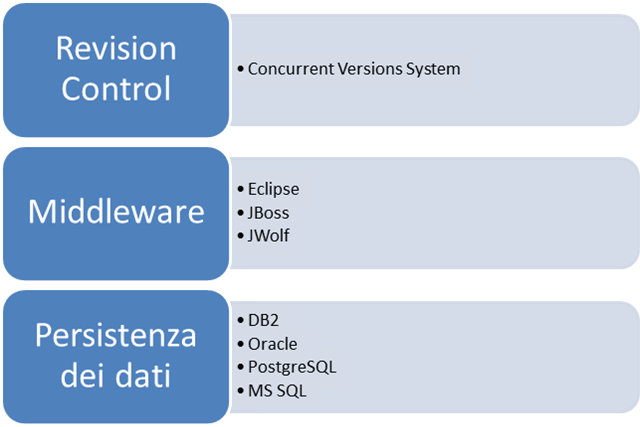
\includegraphics[scale=0.55]{../Logo&Header/tecnologieUsate.png}
\caption{Tecnologie in uso}
\end{figure}


\subsection{Processi interni}
\label{1.4}
Le fasi di sviluppo di un progetto sono costituite da:
\begin{itemize}
\item Coordinamento e Riunioni.
In questa fase vengono pianificate tutte le attività necessarie allo svolgimento del progetto. Gli incontri con i clienti hanno come scopo una efficiente trasmissione di informazioni;
\item Analisi dei requisiti.
L'output dell'attività di analisi è un documento in cui vengono racchiusi tutti i requisiti funzionali, qualitativi, prestazionali e dichiarativi dei quali il prodotto finale dovrà garantirne il soddisfacimento. Il documento serve da input per la fase di progettazione;
\item Progettazione.
Nella fase di progettazione si definiscono le specifiche tecniche delle funzionalità da realizzare. Il risultato di questa fase è il documento di Specifiche Tecniche di Progettazione;
\item Sviluppo.
\'{E} lo stadio esecutivo del progetto con il quale si realizzano i moduli software previsti dal disegno applicativo. In questa fase vengono effettuati test di unità;
\item Test funzionali e di sistema.
I test funzionali hanno lo scopo di verificare che i moduli realizzati durante la fase di codifica rispettino quanto fissato dai requisiti iniziali. Il test di sistema valida il prodotto nella sua interezza;
\item Collaudo con il cliente.
Si tratta di un test di sistema effettuato su un ambiente del cliente e con dati di prova forniti dallo stesso. L'output di questa attività è un verbale che racconta l'esito del collaudo;
\item Documentazione di prodotto.
Questa fase prevede la stesura dei Manuali di Prodotto relativi al software realizzato;\\
\end{itemize}

L'output di ogni fase viene verificato e, se conforme agli standard di qualità dell'azienda, approvato. Altrimenti dovranno essere indicate delle misure correttive per i problemi individuati.\\

In figura 3 vediamo un resoconto delle fasi necessarie allo sviluppo software.
\begin{figure}[H]
\centering
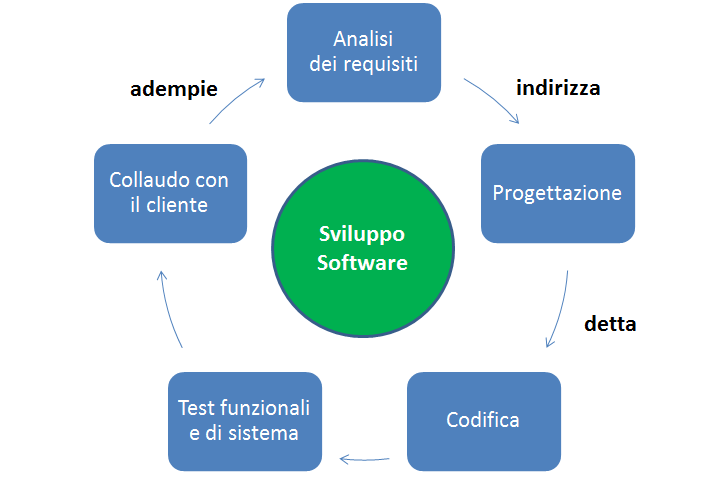
\includegraphics[scale=0.55]{../Logo&Header/sviluppoSoftware.png}
\caption{ Sviluppo Software, ciclo di vita}
\end{figure}

\newpage
\newpage

\section{Progetto aziendale}
\label{2.0}
Questo capitolo ha lo scopo di mostrare al lettore l'ambito in cui si colloca il progetto di stage proposto dall'azienda Corvallis. Inizialmente presento i motivi che hanno portato alla nascità del progetto. A seguire effettuo una panoramica sulla classificazione delle firme statiche. In seguito descrivo il prototipo/classificatore preesistente al progetto di stage. Infine illustro gli obiettivi, le aspettative e i vincoli del progetto aziendale a cui ho preso parte.\\\\
Visti i notevoli vantaggi in termini di incremento dell'efficienza e di riduzione dei costi che la \gls{dematerializzazione} garantisce (risparmio relativo ai costi di stampa, acquisto e manutenzione delle stampanti), nell'ambito delle nuove normative alle banche sarà concesso lo scambio di immagini degli assegni bancari. 

In base a questa premessa l'azienda Corvallis ha intuito che il core di un'applicazione bancaria che accetta lo scambio di immagini degli assegni bancari sarà un classificatore di firme statiche accurato, robusto e affidabile. Conseguentemente ha implementato un prototipo per la classificazione di firme statiche.

\subsection{Introduzione alla classificazione di firme statiche}
\label{2.1}
La firma è un tratto comportamentale di un individuo e costituisce una particolare classe di scrittura dove lettere o parole possono essere non distinguibili. \'{E} considerata un elemento distintivo avente caratteristiche uniche e personali. Accertare in maniera chiara ed univoca il sottoscrittore di un documento avente forza legale (in questo caso assegni bancari) è di fondamentale importanza. Infatti il destinatario deve poter identificare l'identità del mittente (autenticità) e il mittente non deve poter disconoscere un documento da lui firmato (non ripudio). Nasce quindi l'esigenza di distinguere tra firme false e firme autentiche.\\\\
Le difficoltà principali nel classificare le firme autografe sono dovute alle variazioni intrapersonali: le firme di una persona possiedono grande variabilità, dovuta allo stato emotivo dei sottoscrittori oppure alla posizione di raccolta, e di conseguenza, se confrontassimo due esemplari di firma di un firmatario questi non sarebbero identici. Invece l'agevolazione cardinale sta nel fatto che le firme di persone diverse manifestano caratteristiche elementari distinte.\\\\
A seconda del hardware front-end, un sistema di verifica della firma (signature verification system) può essere etichettato come offline o online. Nei sistemi offline la verifica della firma avviene dopo la sottoscrizione della firma. Le uniche informazioni che si possiedono sono di natura statica: l'immagine della firma autografa del sottoscrivente. Al contrario, nei sistemi online, le firme vengono acquisite tramite un dispositivo elettronico (tavoletta grafica) oppure con una penna speciale, capace di memorizzare una sequenza di punti che descrivono velocità, pressione, ritmo, accelerazione e movimento effettuati dal sottoscrittore, non solo l'immagine statica.

\subsubsection{Valutazione delle performance}
\label{2.1.1}
La performance di un sistema di verifica della firma si calcola in base alla percentuale di errori che esso commette nel classificare le firme. Esistono due tipi di errori. Questi vengono riassunti dai seguenti indici:
\begin{itemize}
\item False Acceptance Rate (FAR), indice di accettazione dei falsi, ossia percentuale delle firme false classificate come genuine;
\[FAR =
\frac{nr.\ falsi\ accettati}{nr.\ falsi\ totali}
\]
\item False Rejection Rate (FRR), indice di rifiuto dei genuini, ossia percentuale delle firme genuine classificate come false.
\[FRR =
\frac{nr.\ genuini\ rifiutati}{nr.\ genuini\ totali}
\]
\end{itemize}
Purtroppo i due indici sono inversamente proporzionali: a una diminuzione del FAR corrisponde un aumento del FRR e viceversa a una diminuzione del FRR corrisponde un aumento del FAR. \'{E} evidente quindi che si deve arrivare a un compromesso: minimizzare il FAR conservando un valore tollerabile per il FRR.

Se si eguagliano i due indici si è in presenza di un nuovo indice: Equal Error Rate (EER). L'EER permette di paragonare in modo veloce l'accuratezza dei sistemi di verifica. In generale, più l'indice EER è basso più il sistema è accurato.

Non sorprendentemente, grazie ai dati biometrici che i sistemi di verifica della firma online possiedono in più, essi sono più accurati e affidabili dei sistemi di verifica della firma statica.

\subsubsection{Tipi di falsificazione}
\label{2.1.2}
In letteratura sono stati individuati tre tipi di falsificazione a seconda del grado di preparazione del falsificatore sulla firma che sta cercando di riprodurre:
\begin{itemize}
\item falsificazioni casuali (random forgeries), prodotte senza conoscere né il nome del firmatario né la forma della sua firma;
\item falsificazioni semplici (simple forgeries), prodotte conoscendo il nome del firmatario ma senza avere un esempio della sua firma;
\item falsificazioni accurate (skilled forgeries), prodotte dopo un allenamento con l'obiettivo di imitare la firma originale nel miglior modo possibile.
\end{itemize}
In figura 4 vediamo un esempio di firma genuina e degli esempi di falsificazione della stessa.
\begin{figure}[H]
\centering
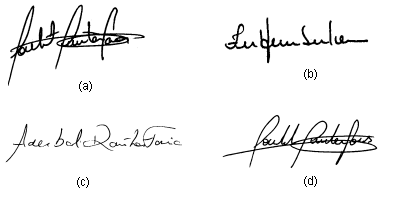
\includegraphics[scale=1.0]{../Logo&Header/esempiForged.png}
\caption{Tipi di falsificazioni:} (a) firma genuina; (b) falsificazione casuale;\\
(c) falsificazione semplice; (d) falsificazione accurata
\end{figure}

\subsubsection{Verifica della firma statica (offline signature verification)}
\label{2.1.3}
La verifica di firme statiche appartiene alla classe di problemi del pattern recognition e un tipico sistema di pattern recognition si compone dai seguenti step \cite{2698894}:
\begin{enumerate}
\item Acquisizione dati, cattura delle immagini firma;
\item Preprocessing, per semplificare le operazioni successive minimizzando la perdita di informazioni;
\item Estrazione delle caratteristiche (feature extraction), riduzione dei dati in input misurando solo determinate caratteristiche (feature) o proprietà;
\item Classificazione (oppure fase di verifica), prendere una decisione (accettare o rifiutare) sulla base dell'adeguatezza dei valori ottenuti dalla fase di feature extraction.
\end{enumerate}
In figura 5 vediamo il workflow generale del processo di verifica della firma statica.
\begin{figure}[H]
\centering
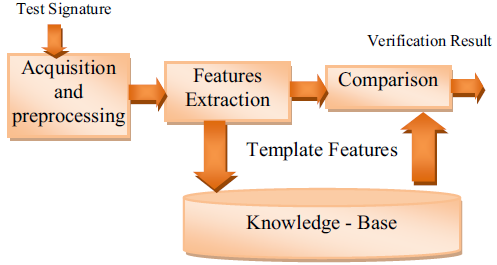
\includegraphics[scale=0.8]{../Logo&Header/generalProcess.png}
\caption{Workflow dei sistemi di verifica della firma statica} Sorgente: \cite{4}
\end{figure}
\subsubsection*{Acquisizione dati}
\label{2.1.3.1}
Le immagini di firma vengono scannerizzate oppure vengono estratte da documenti PDF.
\subsubsection*{Preprocessing}
\label{2.1.3.1}
Il preprocessing della firma è uno step fondamentale necessario a migliorare l'accuratezza dell'estrazione delle caratterisitche e della classificazione. Lo scopo della fase di preprocessing è quello di standardizzare le firme e renderle pronte per la fase di feature extraction.\\ Di seguito elenco alcune delle operazioni di preprocessing più utilizzate:
\begin{itemize}
\item Estrazione della firma (signature extraction);
\item Ritaglio (cropping), l'immagine viene ridotta al rettangolo che circoscrive la firma;
\item Ridimensionamento (resizing), l'immagine della firma viene ridimensionata;
\item Binarizzazione (binarization), conversione da colore a scala di grigi e infine a bianco-nero (binario);
\item Assottigliamento (thinning), assottigliamento del tratto della firma a un pixel per uniformare lo spessore;
\end{itemize}
Un'errata scelta degli algoritmi di preprocessing può comportare una considerevole perdita di informazione.

\subsubsection*{Estrazione delle features}
\label{2.1.3.2}
Il successo di un sistema di verifica della firma dipende fortemente dalla fase di Estrazione delle features. Un metodo ideale di feature extraction prevede l'estrazione di quelle caratteristiche che minimizzano le variazioni intrapersonali presenti nelle firme di un sottoscrittore e massimizzano le variazioni interpersonali presenti nelle firme di due sottoscrittori distinti\cite{2}.\\\\
A seconda della facilità con la quale si possono imitare, le feature possono essere classificate in feature statiche o feature pseudo-dinamiche. La prima categoria contiene caratteristiche percettive e quindi facili da imitare, mentre la seconda categoria contiene caratteristiche poco intuitive e quindi di difficile imitazione\cite{3}.
Segue un elenco stringato delle features più utilizzate in letteratura.\\
Features statiche:
\begin{itemize}
\item Calibre, valore che individua il rapporto tra altezza e larghezza della firma;
\item Proportion, si riferisce alle simmetrie presenti nell'immagine
\item Spacing, valore che individua il numero di blocchi che compongono la firma, se non vi sono spaziature questo valore è uguale a 1;
\item Base behavior, descrive l'angolo di inclinazione della firma in base a un'immaginaria linea orizzontale.
\end{itemize}
Features pseudo-dinamiche:
\begin{itemize}
\item Density of pixels, descrive la larghezza dei tratti, viene considerata "pressione apparente";
\item Distribution of pixels, descrive il numero di pixel neri presenti in uno spazio;
\item Slant, individua informazioni riguardo all'inclinazione del tratto in considerazione;
\item Form, individua informazioni riguardo alla forma del tratto in considerazione;
\end{itemize}
Un'ulteriore suddivisione delle features è dovuta alla segmentazione. In presenza di un'immagine firma segmentata le features possono essere globali (riguardano l'immagine nella sua interezza) o locali (riguardano determinate parti dell'immagine).\\\\
In figura 6 vediamo la panoramica delle features sopra elencate.
%prima era scritto \begin{figure}[h!] per il float default immagini?
\begin{figure}[H]
\centering
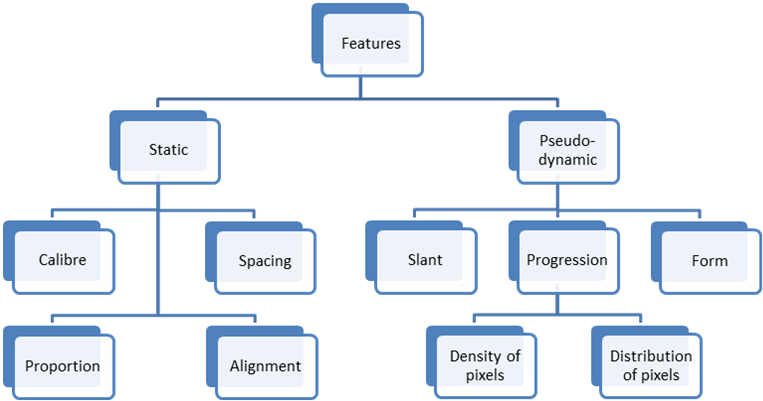
\includegraphics[scale=0.7]{../Logo&Header/featuresStaticPseudoD.png}
\caption{Features statiche e features pseudo-dinamiche}
\end{figure}
\subsubsection*{Classificazione}
\label{2.1.3.2}
L'ultimo step nel processo di verifica dei sistemi offline decide se la firma presa in considerazione è genuina o falsa.\\
In letteratura esistono diversi tipi di approcci al problema della classificazione di firme statiche.\\\\
In figura 7 riporto un grafico riassuntivo degli approcci più utilizzati.\\
\begin{figure}[H]
\centering
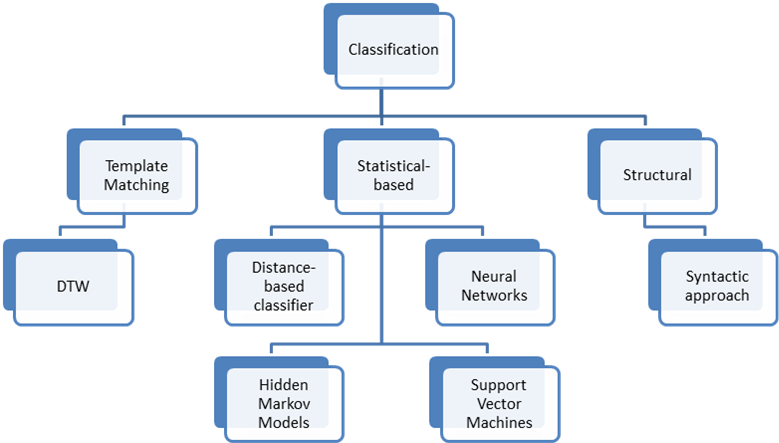
\includegraphics[scale=0.7]{../Logo&Header/classificatori.png}
\caption{Panoramica metodi di classificazione}
\end{figure}
Poiché alcuni dei prossimi argomenti di questa relazione trattano i classificatori di tipo Statistical-based, né spiego la logica.
\subsubsection*{Classificatori Statistical-based}
\label{2.1.3.2}
Nei classificatori di tipo Statistical-based la conoscenza statistica viene utilizzata per usufruire di nozioni come la relazione, la deviazione, tra due o più item per trovare qualche specifica correlazione tra essi. Nei sistemi di verifica della firma, la firma media (template/pattern) viene elaborata a partire da firme collezionate precedentemente (nella fase di training). Questa viene salvata nella "base di conoscenza" e quando si ha in input una firma da classificare viene utilizzato il concetto di correlazione per calcolare la distanza tra la firma da verificare e la firma media per poi decidere se accettarla o rifiutarla.\\\\
Nella prossima sezione descrivo il classificatore di firme statiche implementato dall'azienda Corvallis prima del progetto di stage.
\subsubsection{Prototipo preesistente}
\label{2.1.4}
Il classificatore di firme statiche, implementato dall'azienda, fa parte della categoria Statistical-based. In particolare è un classificatore di tipo Distance-based.\\\\
Il prototipo è in grado di estrarre 21 feature.
Il sistema viene addestrato utilizzando un database di firme. Per ciascun sottoscrittore, un vettore contenente il baricentro di ogni feature (centroid feature vector) viene calcolato utilizzando gli esemplari di firma genuini. Il vettore baricentro costituisce il template delle firme del firmatario. In fase di verifica, per misurare la distanza tra la firma template e la firma da testare, viene adoperata la distanza Euclidea nello spazio delle features.\\
La particolarità di questo sistema sta nel fatto che, per classificare una firma, non si basa soltanto sulla distanza Euclidea ma anche su un meccanismo dei pesi. Si assegna una peso ad ogni feature in base alla variabilità intrapersonale che essa assume tra i prototipi firma di un sottoscrittore. Questa meccanica è descritta meglio nelle sezioni a seguire.\\\\
In figura 8 segue uno schema riassuntivo dei processi interni al classificatore.
\begin{figure}[H]
\centering
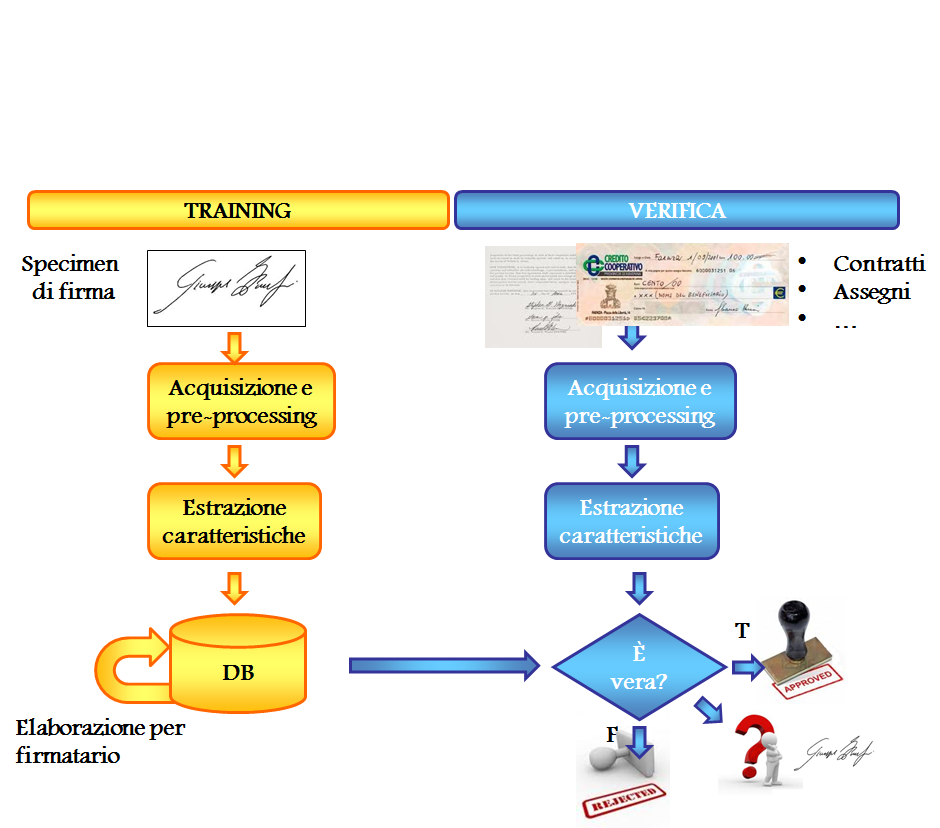
\includegraphics[scale=0.6]{../Logo&Header/processoPrototipoPrees.png}
\caption{Il processo}Sorgente:Corvallis
\end{figure}

\subsubsection*{Fase di training}
\label{2.1.4.1}
Il training prende in input N prototipi di firma genuina, una lista di feature da estrarre e i preprocessing necessari ad ogni feature. Restituisce in output un file contenente quattro attributi per feature, utili in fase di verifica:
\begin{itemize}
\item average, la media di una feature è data dalla somma dei valori che tale feature assume negli N prototipi diviso N:
\[Faverage =
\frac{\sum\limits_{i=1}^N FValPrototipoI}{N}
\]
\item threshold, la soglia di una feature è data dal massimo valore tra la massima distanza del valore della feature dalla media e il 10\% della media:
\[Fthreshold = 
\max \lbrack \max ( |FValPrototipoI - Faverage| ) , ( Faverage * 0.1 )\rbrack
\]
\item weight, il peso di una feature è diverso da utente a utente poiché è inversamente proporzionale alla variabilità della feature rispetto alle altre dell'utente considerato. Il peso di una feature appartiene all'intervallo [0, 1].
\begin{itemize}
\item il peso vale 0 se la deviazione standard è maggiore del 30\% della media;
\item il peso vale 1 se la deviazione standard è uguale a 0;
\item altrimenti:
\[Fweight = \frac{1}{log(minimaDeviazioneStandard)} * log(FdeviazioneStandard)\]
\end{itemize}
con minimaDeviazioneStandard si intende la minima deviazione standard tra tutte le feature considerate; con FdeviazioneStandard si intende la deviazione standard per la feature F.
\item tollerance, il valore della tolleranza è inversamente proporzionale alla variabilità delle feature rispetto alle altre (per un utente specifico). Più una feature è poco variabile più il sistema è tollerante nei suoi confronti in fase di verifica. La tolleranza appartiene all'intervallo [minTol, maxTol]; minTol e maxTol sono due dei parametri che possono essere impostati a priori. La tolleranza vale maxTol se il peso della feature corrente è massimo (Fweight=1). Altrimenti, data la lista ordinata dei pesi, la si può calcolare con la seguente formula:
\[Ftollerance=maxTol - i * \frac{maxTol - minTol}{N-1}\]
i è la posizione i-esima nella lista ordinata dei pesi. Poiché il peso e la tolleranza sono direttamente proporzionali essi scalano insieme.
\end{itemize}
In figura 9 segue uno schema riassuntivo delle operazioni eseguite durante la fase di training.
\begin{figure}[H]
\centering
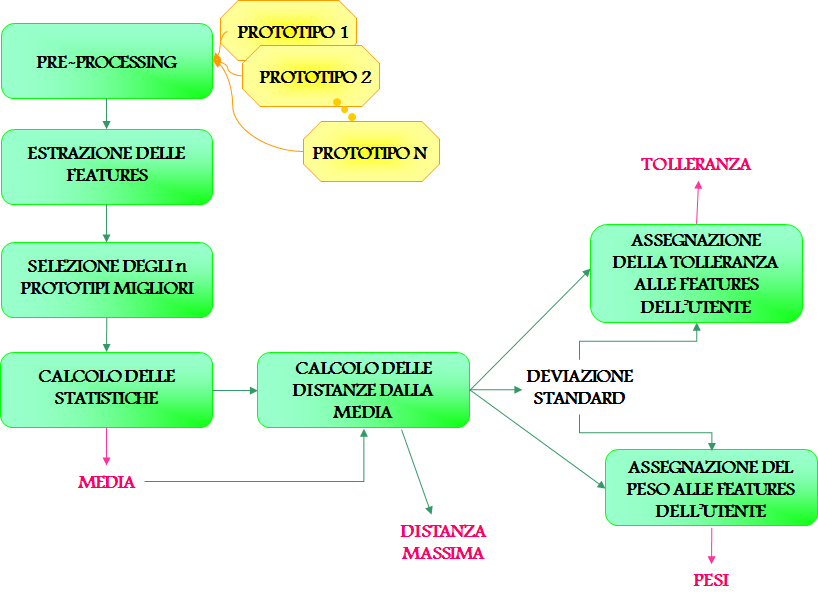
\includegraphics[scale=0.6]{../Logo&Header/trainingFirmatario.png}
\caption{Training per firmatario}Sorgente: Corvallis
\end{figure}

\subsubsection*{Fase di verifica}
\label{2.1.4.2}
Il processo di verifica prevede i seguenti step:
\begin{enumerate}
\item Estrazione delle feature della firma di cui si vuole verificare l’autenticità, secondo la lista feature e preprocessing dell’utente che si vuole personificare;
\item Assegnazione dei voti;
\item Calcolo dei punteggi;
\item Calcolo della confidenza.
\end{enumerate}
\subsubsection*{Assegnazione dei voti}
\label{2.1.4.3}
Il valore di ogni feature estratta dalla firma da verificare viene confrontato con la media corrispondente (presa dal feature centroid vector). In base a quanto si scosta dalla media, ad ogni feature viene assegnato un voto nell'intervallo [-1, 1].
\begin{itemize}
\item il voto è uguale a 1 (voto massimo possibile) quando la differenza tra il valore della feature e la relativa media salvata è uguale a 0, ossia il valore della feature è uguale alla media salvata.
\item il voto è uguale a -1 (voto minimo possibile) quando la differenza tra il valore della feature e la relativa media salvata è maggiore o uguale a due volte la soglia.
\item altrimenti il voto viene assegnato secondo una funzione lineare:
\[Fvoto=\frac{Fthreshold-|FVal-Faverage|}{Fthreshold}\]
\end{itemize}
\subsubsection*{Calcolo dei punteggi}
\label{2.1.4.4}
Il core del sistema classifica le firme in base al punteggio che queste riescono a raggiungere. Il punteggio massimo raggiungibile è chiaramente la somma dei pesi delle feature. Vediamo ora come si calcola il singolo punteggio che poi andrà a costituire parte del punteggio finale.
\[Fpunteggio=Fvoto * Fweight\]
Fvoto è il voto assegnato alla feature F e Fweight è il peso della feature F calcolato durante il training.
\subsubsection*{Calcolo della confidenza}
\label{2.1.4.5}
La decisione finale è data dal valore della confidenza. Se il valore della confidenza è maggiore di 50, la firma viene accettata altrimenti rifiutata. Il calcolo della confidenza è dato da:
\[Confidenza = \frac{0.5+\sum\limits_{i=1}^M FIpunteggio}{2*\sum\limits_{i=1}^M FIweight} * 100\]
M indica il numero di feature prese in considerazione.\\\\
In figura 10 segue uno schema riassuntivo delle operazioni eseguite durante la fase di verifica.
\begin{figure}[H]
\centering
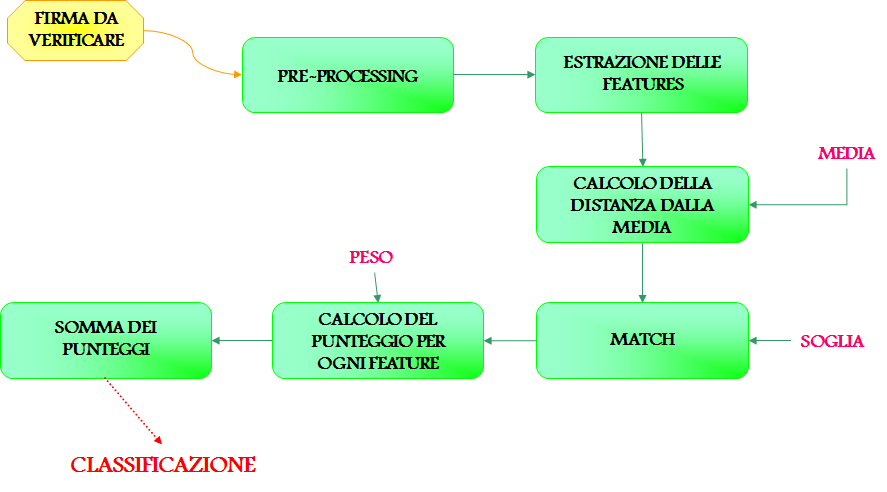
\includegraphics[scale=0.5]{../Logo&Header/verificaFirma.png}
\caption{Verifica firma}Sorgente: Corvallis
\end{figure}
\subsubsection*{Performance}
\label{2.1.4.6}
In tabella 1 vengono riportati i risultati di alcuni test.
\begin{table}[H]
  \label{tbl:excel-table}
  \centering
  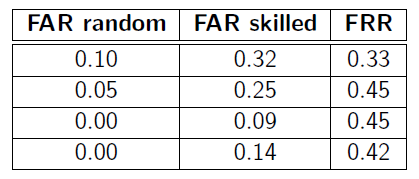
\includegraphics[scale=0.7]{../Logo&Header/overallResult.png}
  \caption{Risultati test prototipo preesistente}
\end{table}
\subsubsection*{Tecnologie impiegate}
\label{2.1.4.7}
Il prototipo è stato scritto in Java, utilizzando l'ide Eclipse. Le librerie utilizzate per l'elaborazione delle immagini sono ImageJ e ImageMagick. Il versionamento del codice è stato effettuato grazie a Content Versioning System (CVS).\\\\
La prossima sezione introduce il progetto di stage a cui ho preso parte.
\subsection{Obiettivi}
\label{2.2}
L'obiettivo principale dello stage è lo studio e l'implementazione di un nuovo classificatore di firme statiche, sempre nell'ambito dei classificatori Statistical-based. Uno degli obiettivi secondari è testare approfonditamente il software preesistente per identificare le eventuali cause di un bug che rende la classificazione attuale dipendente dalla risoluzione del dispositivo di cattura. L'obiettivo ultimo è quello di valutare le performance del nuovo classificatore e di studiare una modalità di unione delle classificazioni dei due prototipi in modo da aumentare l'accuratezza globale del sistema di verifica delle firme statiche.
\subsection{Aspettative}
\label{2.3}
L'azienda si aspetta che l'obiettivo principale venga raggiunto.
\subsection{Vincoli}
\label{2.4}
Non sono stati imposti vincoli particolari per quanto riguarda lo svolgimento del progetto di stage. I vincoli imposti sono:
\begin{itemize}
\item utilizzare il linguaggio Java per l'implementazione del prototipo
\item fornire documentazione adeguata sul prototipo implementato
\item utilizzare le librerie ImageJ e/o ImageMagick per l'elaborazione delle immagini
\item lo studio di nuovi metodi di classificazione deve avvenire sempre nell'ambito dei classificatori Statistical-based
\end{itemize}

\newpage

\section{Attività di stage}
\label{3.0}
Questo capitolo descrive le scelte operative effettuate, i problemi incontrati, gli effetti che questi ultimi hanno avuto sulla pianificazione stilata dal tutor aziendale e le soluzioni adottate per raggiungere gli obiettivi del progetto di stage. Per prima cosa introduco la pianificazione originale. Successivamente riporto i requisiti che il nuovo prototipo/classificatore dovrà soddisfare. In seguito illustro le decisioni prese in fase di progettazione. In conclusione spiego qualche particolare implementativo.
\subsection{Pianificazione}
\label{3.1}

\begin{figure}[H]
\centering
\noindent\makebox[\textwidth]{%
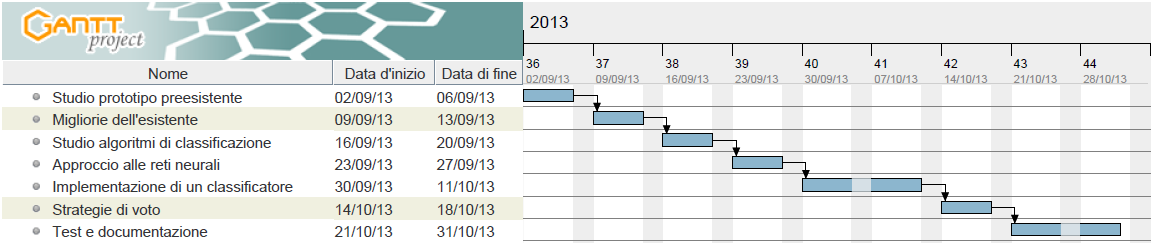
\includegraphics[scale=0.6]{../capitolo3img/pianificazioneIniziale.png}}
\caption{Pianificazione iniziale}
\end{figure}

\subsection{Analisi}
\label{3.2}
I requisiti saranno atomici, chiari,...blblAnalyzing requirements: determining whether the stated requirements are clear, complete, consistent and unambiguous, and resolving any apparent conflicts.
\subsubsection{Ricerca di migliorie del prototipo preesistente}
\label{3.2.1}

\subsubsection{Scelta di un nuovo classificatore di firme statiche}
\label{3.2.2}

\subsubsection{Requisiti}
\label{3.2.3}
Dato un numero di forme genuine, una fase di training, il prodotto deve essere in grado di classificare firme che non ha mai visionato in modo corretto.

UC 1 : Il sistema deve essere in grado di classificare in modo corretto immagini di firma autografa in seguito a una fase di training.

UC 1.1 Il sistema deve essere in grado di eseguire il training su un database di firmatari, dato un certo numero di firme genuine per firmatario.

UC 1.1.1 Il sistema deve essere in grado di effettuare preprocessings su un'immagine firma caricata precedentemente.

UC 1.1.2 Il sistema deve essere in grado di effettuare feature extraction su un'immagine firma caricata precedentemente.

UC 1.1.3 Il sistema deve essere in grado di [qui entra in gioco il statistical based classifier] 

UC 1.1.4 Il sistema deve essere in grado di caricare in memoria l'immagine di una firma. (eheeh che tipo di immagine?)

UC 1.2 Il sistema deve essere in grado di confrontare una firma con il template elaborato in fase di testing.


Qualitativo? deve rispondere in modo corretto l'80\% delle volte!

terminologia adottata sui requisiti?
i requisiti sono gerarchici, l'indice indica il padre 
\subsection{Progettazione}
\label{3.3}
MVC (model firme dentro il file system, view la gui, controller trainer tester, elaborazione immagini, preprocessings...)


Tracciamento? Progettazione, riutilizzo(sodisfatto utilizzando moduli del prototipo preesistente) di alcune funzionalità, tipo preprocessings..., però il CoG segmentation non c'era, e feature extraction : slant, dct ...

\subsection{Implementazione}
\label{3.4}
\newpage

\section{Valutazione retrospettiva}
\label{4.0}

\subsection{Copertura dei requisiti}
\label{4.1}

\subsubsection{Possibili sviluppi alle attività svolte}
\subsection{Conoscenze acquisite}

\label{4.2}
\subsection{Distanza tra conoscenze richieste e conoscenze possedute}

\label{4.3}
\newpage

%\subsection*{Glossario}
\printglossaries
\addcontentsline{toc}{section}{Glossario}
\label{5.0}

\newpage
%\subsection*{Riferimenti}
\begin{thebibliography}{1}
\bibitem{2698894} Hemanta Saikia, Kanak Chandra Sarma {\em Approaches and issues in Offline Signature Verification System}.
\bibitem{2} Battista L., Rivard D., Sabourin R., Granger E., Maupin P., {\em State of the art in off-line signature verification}.
\bibitem{3} Justino, Yacoubi, Bortolozzi, Sabourin {\em An Off-Line Signature Verification System Using HMM and Graphometric Features}.
\bibitem{4} Yazan M. Al-Omari, Khairuddin Omar {\em State-of-the-Art in Offline Signature Verification System}.
\end{thebibliography}
\addcontentsline{toc}{section}{Riferimenti}
\label{6.0}

\newpage




\end{document}
